\documentclass[12pt]{report}

% General includes
\usepackage{amsfonts, amssymb, amsmath}
\usepackage{graphicx}
\usepackage{float}
\usepackage{color, soul}
\usepackage{hyperref}

% Font settings
%\renewcommand\familydefault{\sfdefault}
\usepackage{palatino}  % serif
\usepackage{helvet}    % sans-serif
\usepackage{courier}   % typewriter
\usepackage{euler}     % math mode

% Margin and paragraph indent
\usepackage[margin=1.0in]{geometry}
\usepackage{parskip}

\begin{document}
\begin{titlepage}
	\centering
	\vspace{1cm}
	{\scshape\Large ESE 370: Circuit-Level Optimization for Digital Systems\par}
	\vspace{1.5cm}
	{\huge\bfseries Project 2 Milestone: FIFO Queue\par}
	\vspace{2cm}
	{\Large\itshape Mauricio Mutai, Jack Harkins\par}
	\vfill
	Instructor: Dr. Tania Khanna\par
	TA: Martin Deng\par
	Date: 11/26/16

	\vfill

% Bottom of the page
	{\large \today\par}
\end{titlepage}

\section*{Bitline Capacitance}
\hl{TODO}

\section*{Circuit Schematics}
\hl{TODO}
\subsection*{Memory Column Driver Schematic}

\subsection*{Sized Memory Cell Schematic}

\subsection*{Tri-State Buffer Schematic}

\subsection*{Tri-State Inverter Schematic}


\section*{Reading and Writing (Cell)}
\hl{TODO}
\subsection*{Test Cases to Consider}

\subsection*{Writing 0 and Reading 0}
\begin{figure}[H]
  \centering
    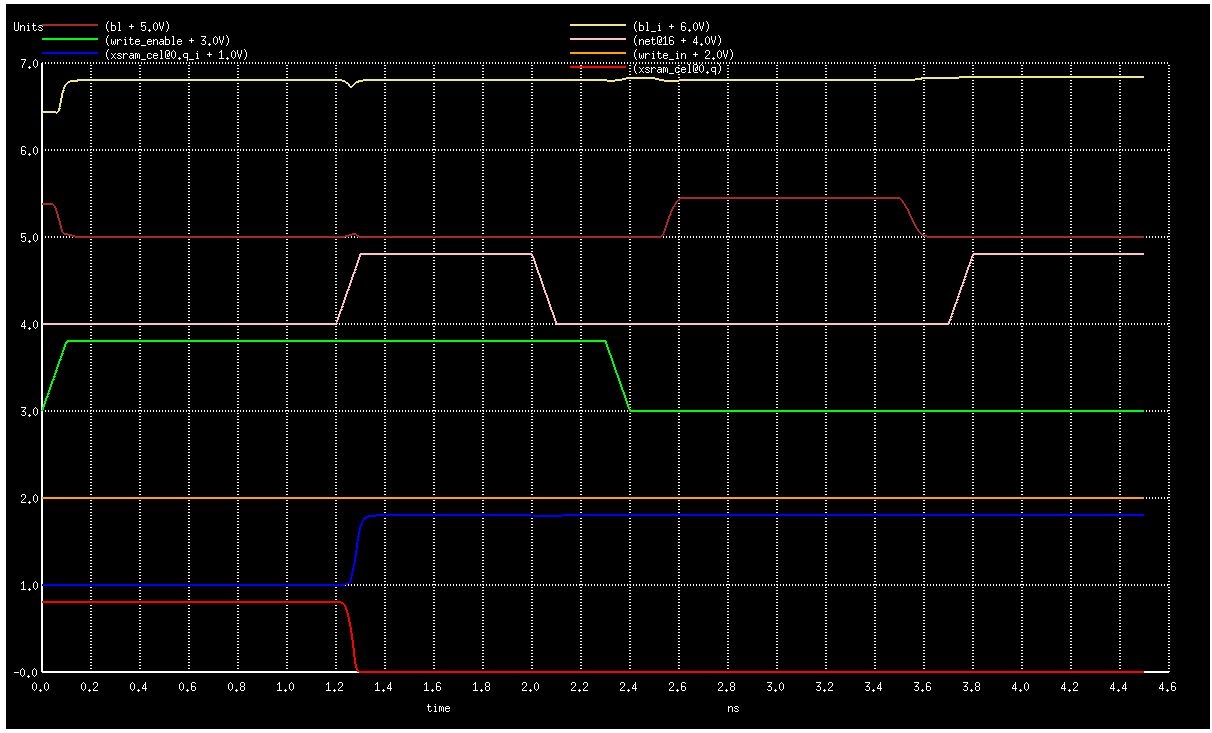
\includegraphics[width=1.0\textwidth]{write_0_then_read_0.png}
  \caption{Writing 0 and then reading 0}
  \label{fig:write_0_then_read_0}
\end{figure}

\subsection*{Writing 1 and Reading 1}
\begin{figure}[H]
  \centering
    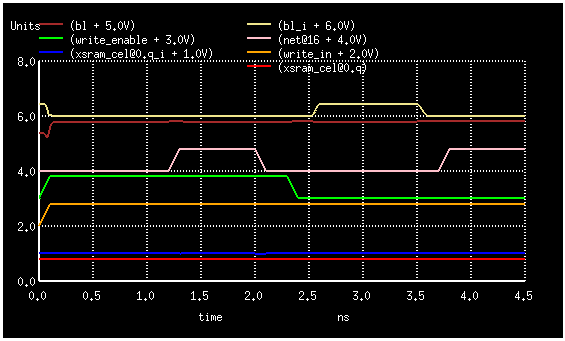
\includegraphics[width=1.0\textwidth]{write_1_then_read_1.png}
  \caption{Writing 1 and then reading 1}
  \label{fig:write_1_then_read_1}
\end{figure}

\subsection*{Writing 0}
\begin{figure}[H]
  \centering
    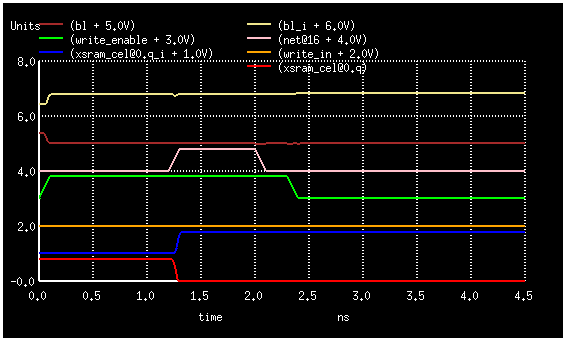
\includegraphics[width=1.0\textwidth]{write_1_then_write_0.png}
  \caption{Writing 0}
  \label{fig:write_1_then_write_0}
\end{figure}

\subsection*{Writing 1}
\begin{figure}[H]
  \centering
    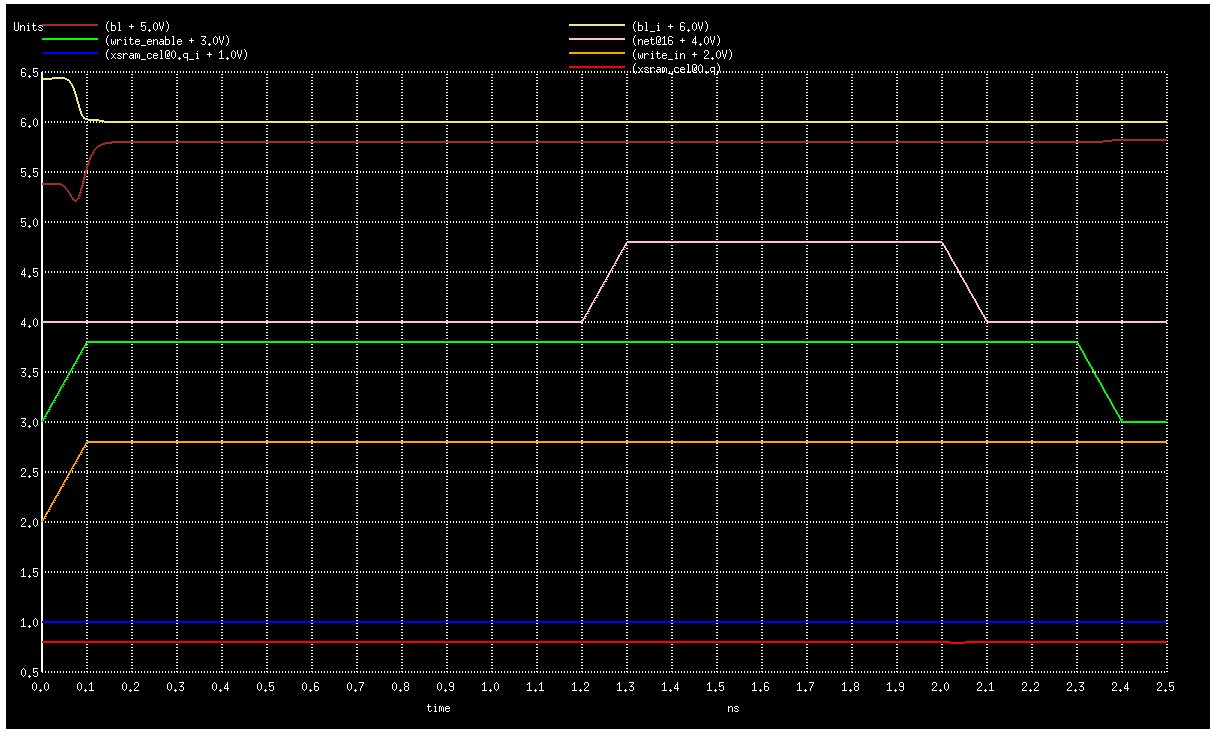
\includegraphics[width=1.0\textwidth]{write_1_then_write_1.png}
  \caption{Writing 1}
  \label{fig:write_1_then_write_1}
\end{figure}

\subsection*{Writing 0 and Writing 1}
\begin{figure}[H]
  \centering
    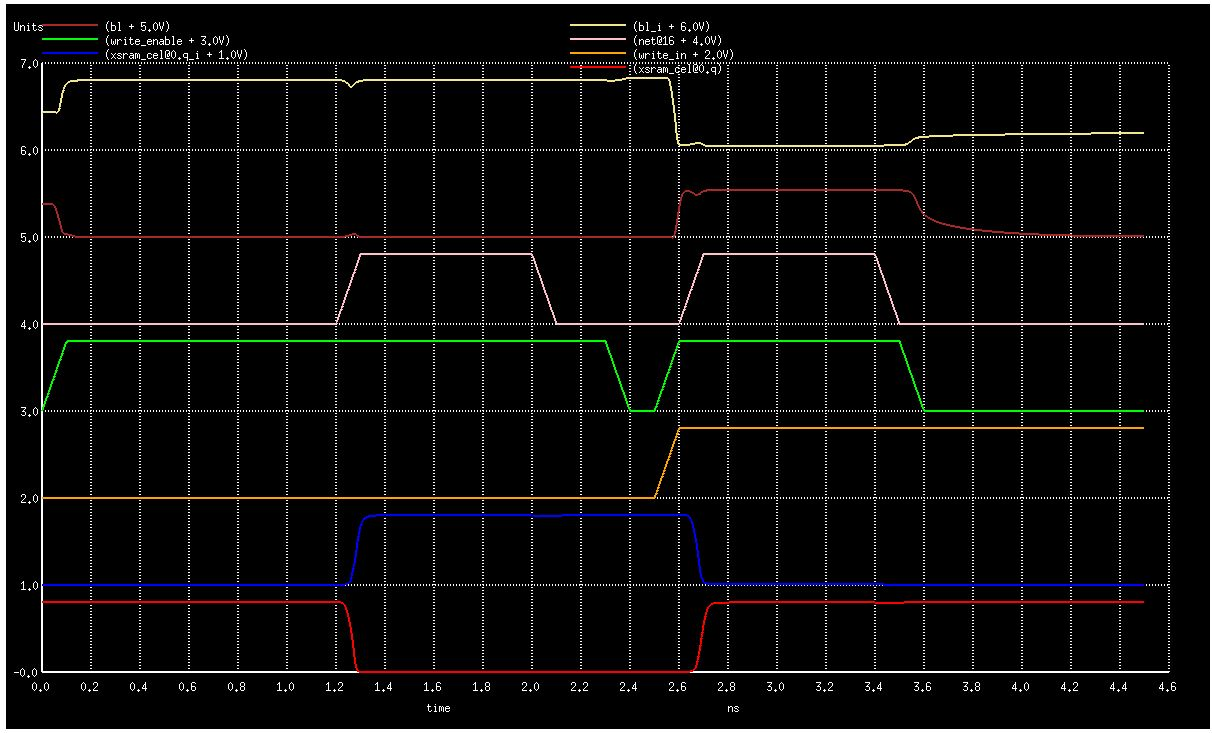
\includegraphics[width=1.0\textwidth]{write_0_then_write_1.png}
  \caption{Writing 0, then writing 1}
  \label{fig:write_0_then_write_1}
\end{figure}

\subsection*{Writing 0 and Writing 0}
\begin{figure}[H]
  \centering
    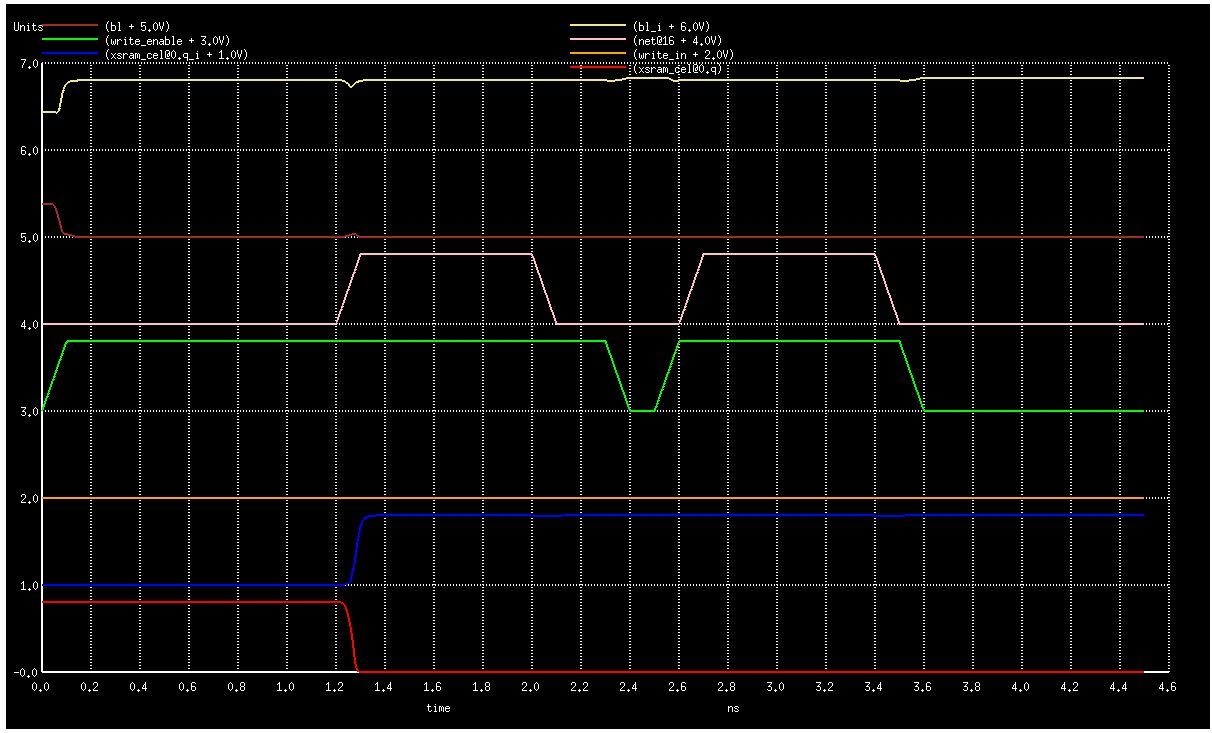
\includegraphics[width=1.0\textwidth]{write_0_then_write_0.png}
  \caption{Writing 0, then writing 0}
  \label{fig:write_0_then_write_0}
\end{figure}

\section*{Constraints on Write Timing, Full FIFO Design}
\hl{TODO}

\end{document}
